Apart from the \acs{SEP}, the long lasting \ac{GCR} and the albedo protons which are the products of the interaction between \ac{GCR} and lunar regolith are another two important components of the plasma environment and radiation hazard on the lunar surface. [citation]
The \ac{GCR} are the higher energetic particle with the energy above ten of MeV/nuc
Those energetic particle oriented from the supernovae remanent outside of the solar system and accelerted to few. GCE from outside of Solar system, accelerated by the shock wave.
The most dominant component are the protons which consist of 98\% of the GCR particles.

The When those higher particle arrived at the lunar surface, the secondary and albedo protons are generated.



From 2019.1 to 2020.7, apart from the SEP event that we studied in the last chapter, no SEPs arrived on the lunar surface during this period, hence it is a good opportunity to study the \acs{GCR} without the interference of the solar energetic particle.

At the sametime, benefit from the advanced structure of \ac{LND}'s charged particle telescope, we design a new data product after LND delivered and launched to the lunar surface. Such a data products allow us measure the flux of albedo proton around few tens of MeV.

\textit{Overview of the key results}
Below we brief summarized the key obseravtions and the 
As the first such measurements ever on the lunar surface, LND provide the unique observation of the quite time spectra of lower energy cosmic ray, 

\begin{itemize}
    \item The LND measurement are consistent with SOHO/EPHIN measurement between 10 - 50 MeV. 
    \item The comparison between measurement and model observations indicates the underestimation of the CREME model during the last solar minimum
    \item The albode proton measurement of LND is consistent with the albedo proton measurements from LRO/CRATER, and also consistent with the model prediction by the REDmoon model
\end{itemize}



The following article is reproduced from \textcite{Xu-2022-LND-GCRalbedo}, which is an open-access article reproducted under the terms of 
the CC-BY license. The supplement material including the configuration changes of LND up to now and the data we used in the main content is attached afterward. 
\\

\noindent\pubcite{Xu-2022-LND-GCRalbedo}\\
\strut\hfill Own contribution: 90\%

\newpage
\newcounter{includepdfpageFrontierTwentyTwo}

\addtocounter{subsection}{1}
\setcounter{subsubsection}{1} 
\phantomsection
\addcontentsline{toc}{subsection}{\arabic{chapter}.\arabic{section}.\arabic{subsection} Primary and albedo protons detected by the Lunar Lander Neutron and Dosimetry experiment on the lunar farside(Publication Frontier in Astronomy and Space Sciences 2022)}
%
\phantomsection
\addcontentsline{toc}{subsubsection}{\arabic{chapter}.\arabic{section}.\arabic{subsection}.\arabic{subsubsection} Introduction}
\label{sec:paper_xu2022}
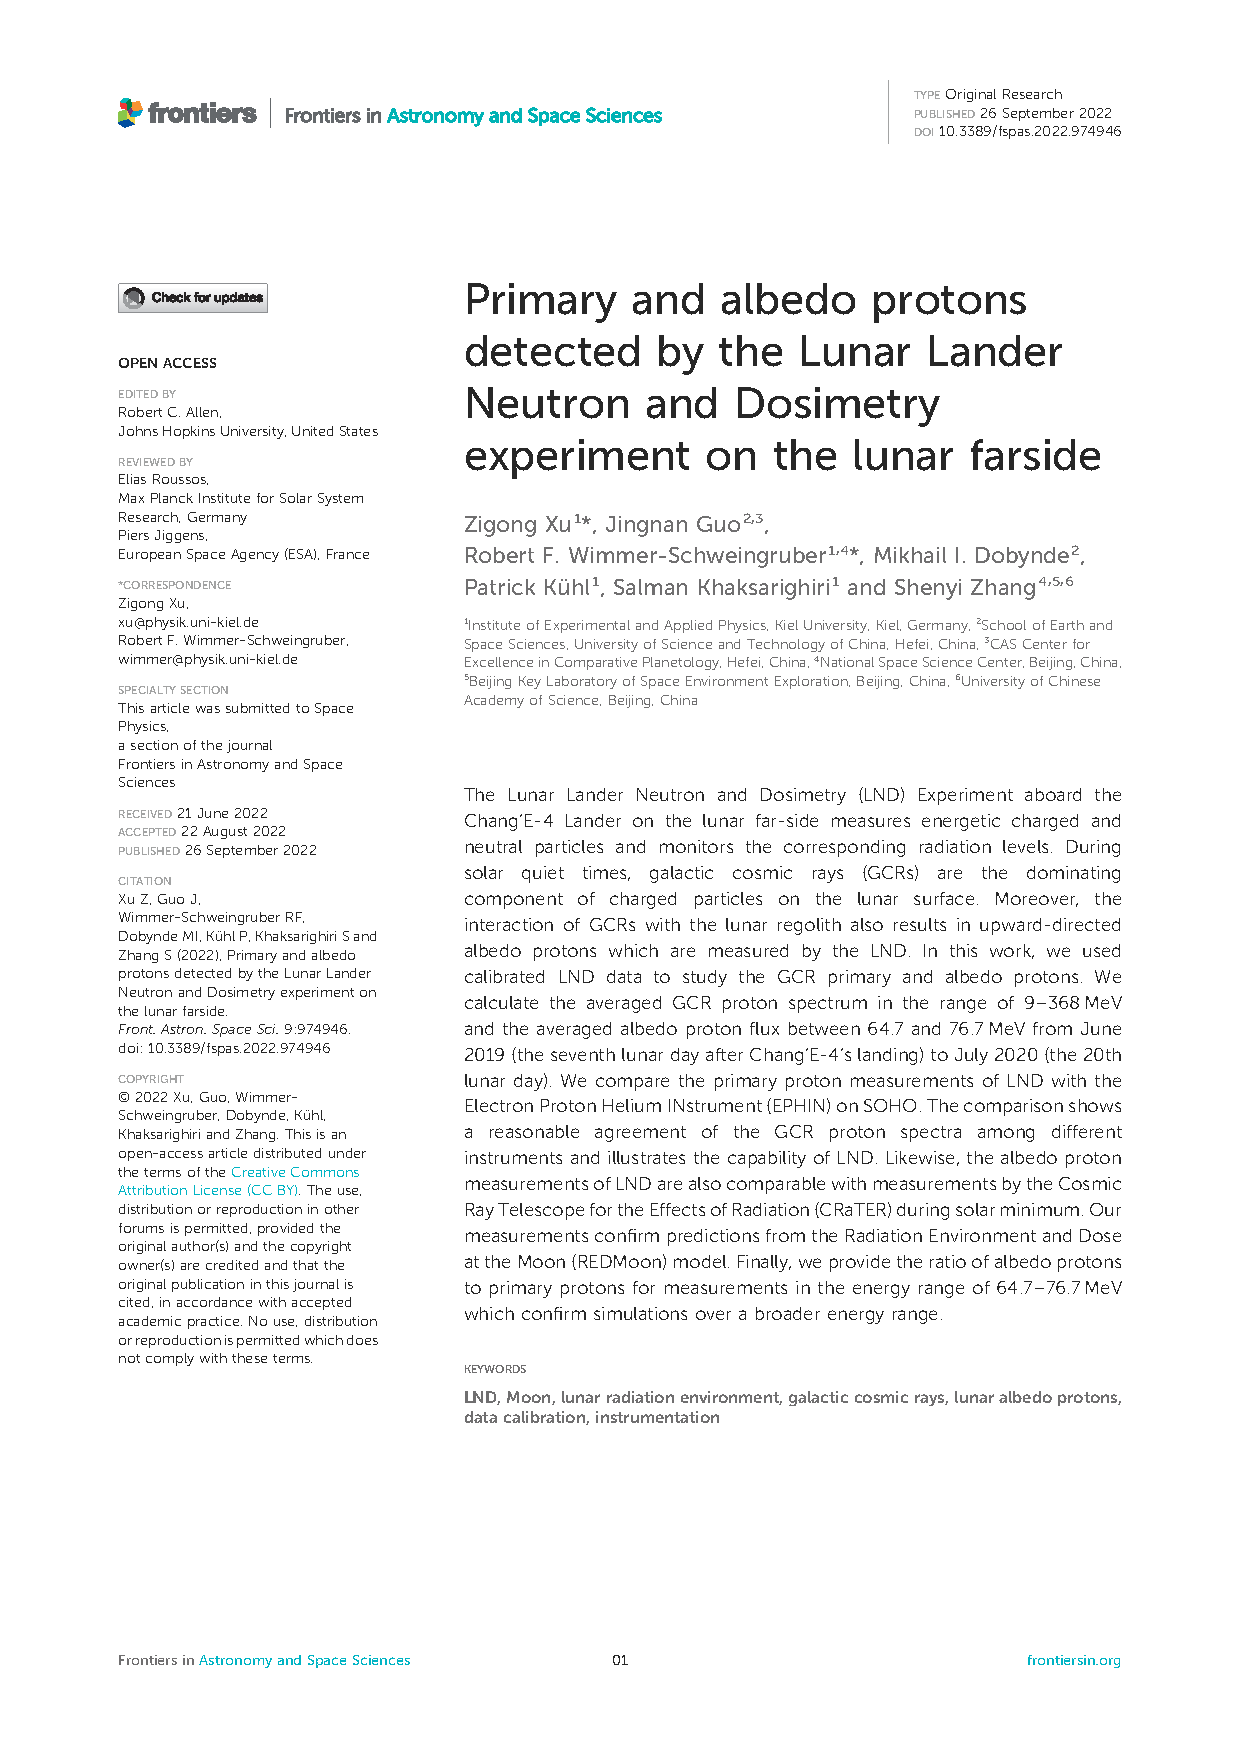
\includepdf[pages={1-3}, link, linkname=paper_xu2022, scale=.9, pagecommand={\refstepcounter{includepdfpageFrontierTwentyTwo}\label{paper_xu2022.\theincludepdfpageFrontierTwentyTwo}}]{publications/Xu_et_al_2022_Frontier.pdf}
%
\addtocounter{subsubsection}{1} 
\phantomsection
\addcontentsline{toc}{subsubsection}{\arabic{chapter}.\arabic{section}.\arabic{subsection}.\arabic{subsubsection} Preparation of LND data}
\includepdf[pages={4-8}, link, linkname=paper_xu2022, scale=.9, pagecommand={\refstepcounter{includepdfpageFrontierTwentyTwo}\label{paper_xu2022.\theincludepdfpageFrontierTwentyTwo}}]{publications/Xu_et_al_2022_Frontier.pdf}
%
\addtocounter{subsubsection}{1} 
\phantomsection
\addcontentsline{toc}{subsubsection}{\arabic{chapter}.\arabic{section}.\arabic{subsection}.\arabic{subsubsection} Measurements and comparison with model}
\includepdf[pages={9-11}, link, linkname=paper_xu2022, scale=.9, pagecommand={\refstepcounter{includepdfpageFrontierTwentyTwo}\label{paper_xu2022.\theincludepdfpageFrontierTwentyTwo}}]{publications/Xu_et_al_2022_Frontier.pdf}
%
\addtocounter{subsubsection}{1} 
\phantomsection
\addcontentsline{toc}{subsubsection}{\arabic{chapter}.\arabic{section}.\arabic{subsection}.\arabic{subsubsection} Summary, discussion and conclusion}
\includepdf[pages={12}, link, linkname=paper_xu2022, scale=.9, pagecommand={\refstepcounter{includepdfpageFrontierTwentyTwo}\label{paper_xu2022.\theincludepdfpageFrontierTwentyTwo}}]{publications/Xu_et_al_2022_Frontier.pdf}
%
\addtocounter{subsubsection}{1} 
\phantomsection
\addcontentsline{toc}{subsubsection}{\arabic{chapter}.\arabic{section}.\arabic{subsection}.\arabic{subsubsection} References}
\includepdf[pages={13-14}, link, linkname=paper_xu2022, scale=.9, pagecommand={\refstepcounter{includepdfpageFrontierTwentyTwo}\label{paper_xu2022.\theincludepdfpageFrontierTwentyTwo}}]{publications/Xu_et_al_2022_Frontier.pdf}
%
\addtocounter{subsubsection}{1} 
\phantomsection
\addcontentsline{toc}{subsubsection}{\arabic{chapter}.\arabic{section}.\arabic{subsection}.\arabic{subsubsection} Supplement material}
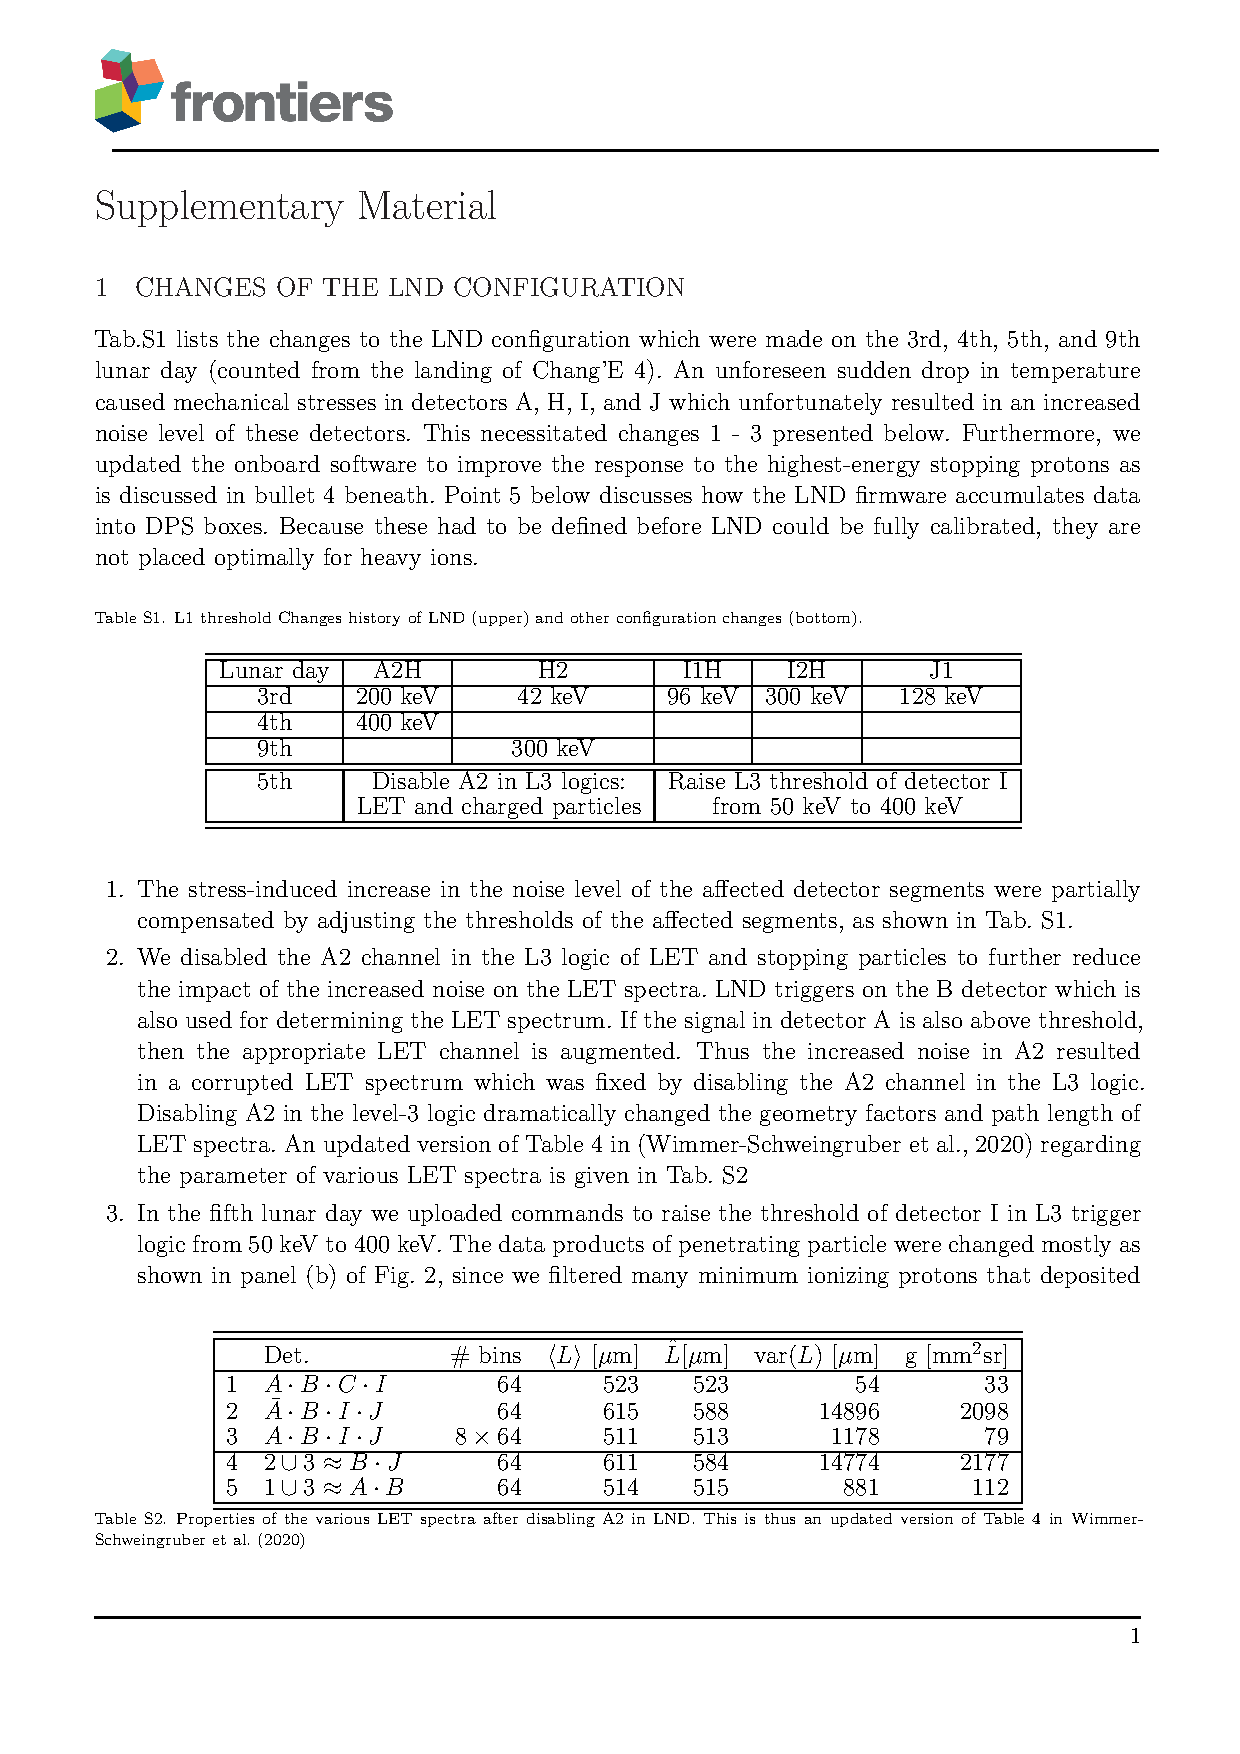
\includepdf[pages={1-3}, link, linkname=paper_xu2022, scale=.9, pagecommand={\refstepcounter{includepdfpageFrontierTwentyTwo}\label{paper_xu2022.\theincludepdfpageFrontierTwentyTwo}}]{publications/Xu_et_al_2022_frontier_appendix.pdf}